\clearpage
\section{Lösungskonzept}\label{sec:Loesungskonzept}
In Abbildung \ref{img:Grobkonzept} ist das Blockschaltbild ersichtlich, welches alle Teilsysteme und Einheiten darstellt. Es ist modular gegliedert und bietet eine Übersicht der Schnittstellen zwischen den einzelnen Modulen. 

Das Lösungskonzept besteht aus physikalisch getrennten Systemen, dem \textit{Universal Peripherial Node} (UPN), dem \textit{Gateway Interface System} (GIS), dem \textit{Human Machine Interface} (HMI) und über das Internet verbundene Webserver, im Konzept als \textit{Platform Bindings} bezeichnet.  

Der \textit{UPN} beinhaltet einen \textit{Bluetoot Mesh Node} (BMN), welcher die Anbindung an das Mesh Netzwerk ermöglicht. Als Stromversorgung dient das \textit{Power Storage System} (PSS), sowie das \textit{Energy Harvesting System} (EHS). Diese Systeme verfügen über externe angebundene Energiequellen (z.B. Solarzellen). Zusätzlich werden die Aktoren und Sensoren des \textit{UPN} über eine \textit{Universal Peripherial Unit} (UPU) angesteuert bzw. eingelesen.

Als Zentrale Einheit des \textit{GIS} dient das \textit{Central Control System} (CCS). Zur Anbindung an das Mesh Netzwerk steht ebenfalls ein \textit{BMN} zur Verfügung. Die Stromversorgung erfolgt über das lokale Stromnetz mithilfe eins Netzteils. Zusätzlich wird die Internetverbindung über das \textit{Mobile Network Interface} (MNI) abgesichert. 

Das \textit{HMI} bildet die Benutzerschnittstelle über ein internetfähiges Gerät. Es kommuniziert mittels WLAN/LAN mit dem \textit{GIS}. Über dieses Gerät kann der Status visualisiert, sowie die Konfigurationen durchgeführt werden.



\begin{figure}
	\centering
	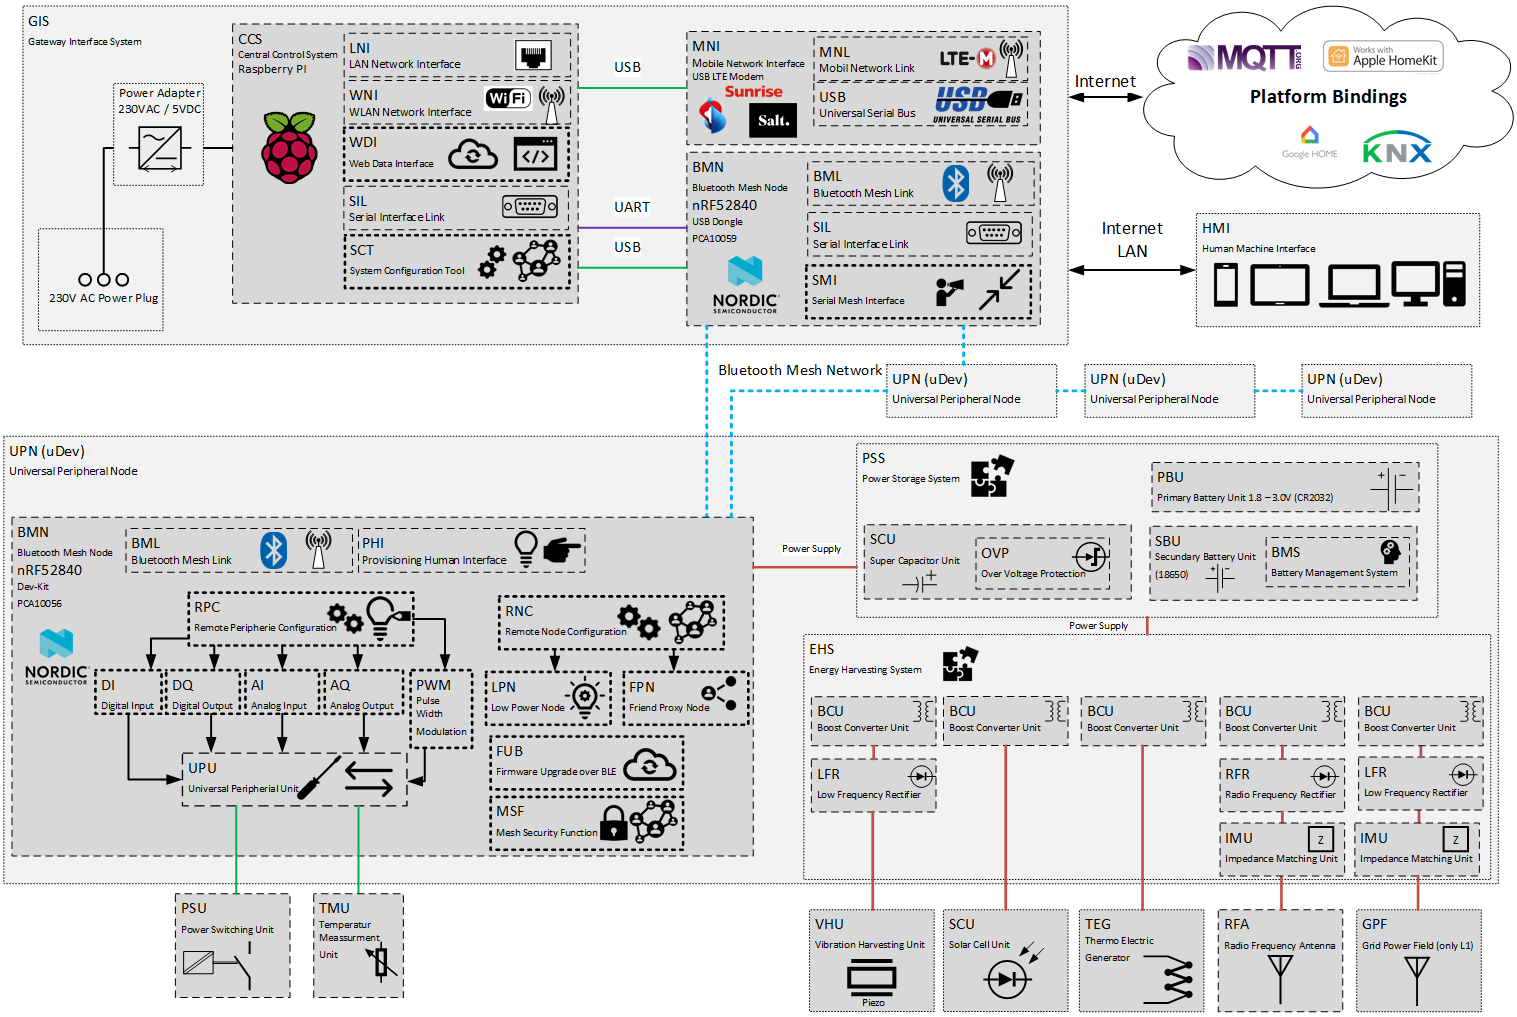
\includegraphics[scale=0.58,angle=90]{19HS-pro5E-TeamBlau_Grobkonzept_04102019_ohne_Rahmen.png}
	\caption{Blockschaltbild des Lösungskonzepts}
	\label{img:Grobkonzept}
\end{figure} 








